\documentclass{standalone}
\usepackage[T1]{fontenc}
\usepackage[utf8]{inputenc}
\usepackage[usenames,dvipsnames]{xcolor}
\usepackage{tikz}
\usetikzlibrary{plotmarks}
\usetikzlibrary{shapes,snakes,arrows}
\begin{document}
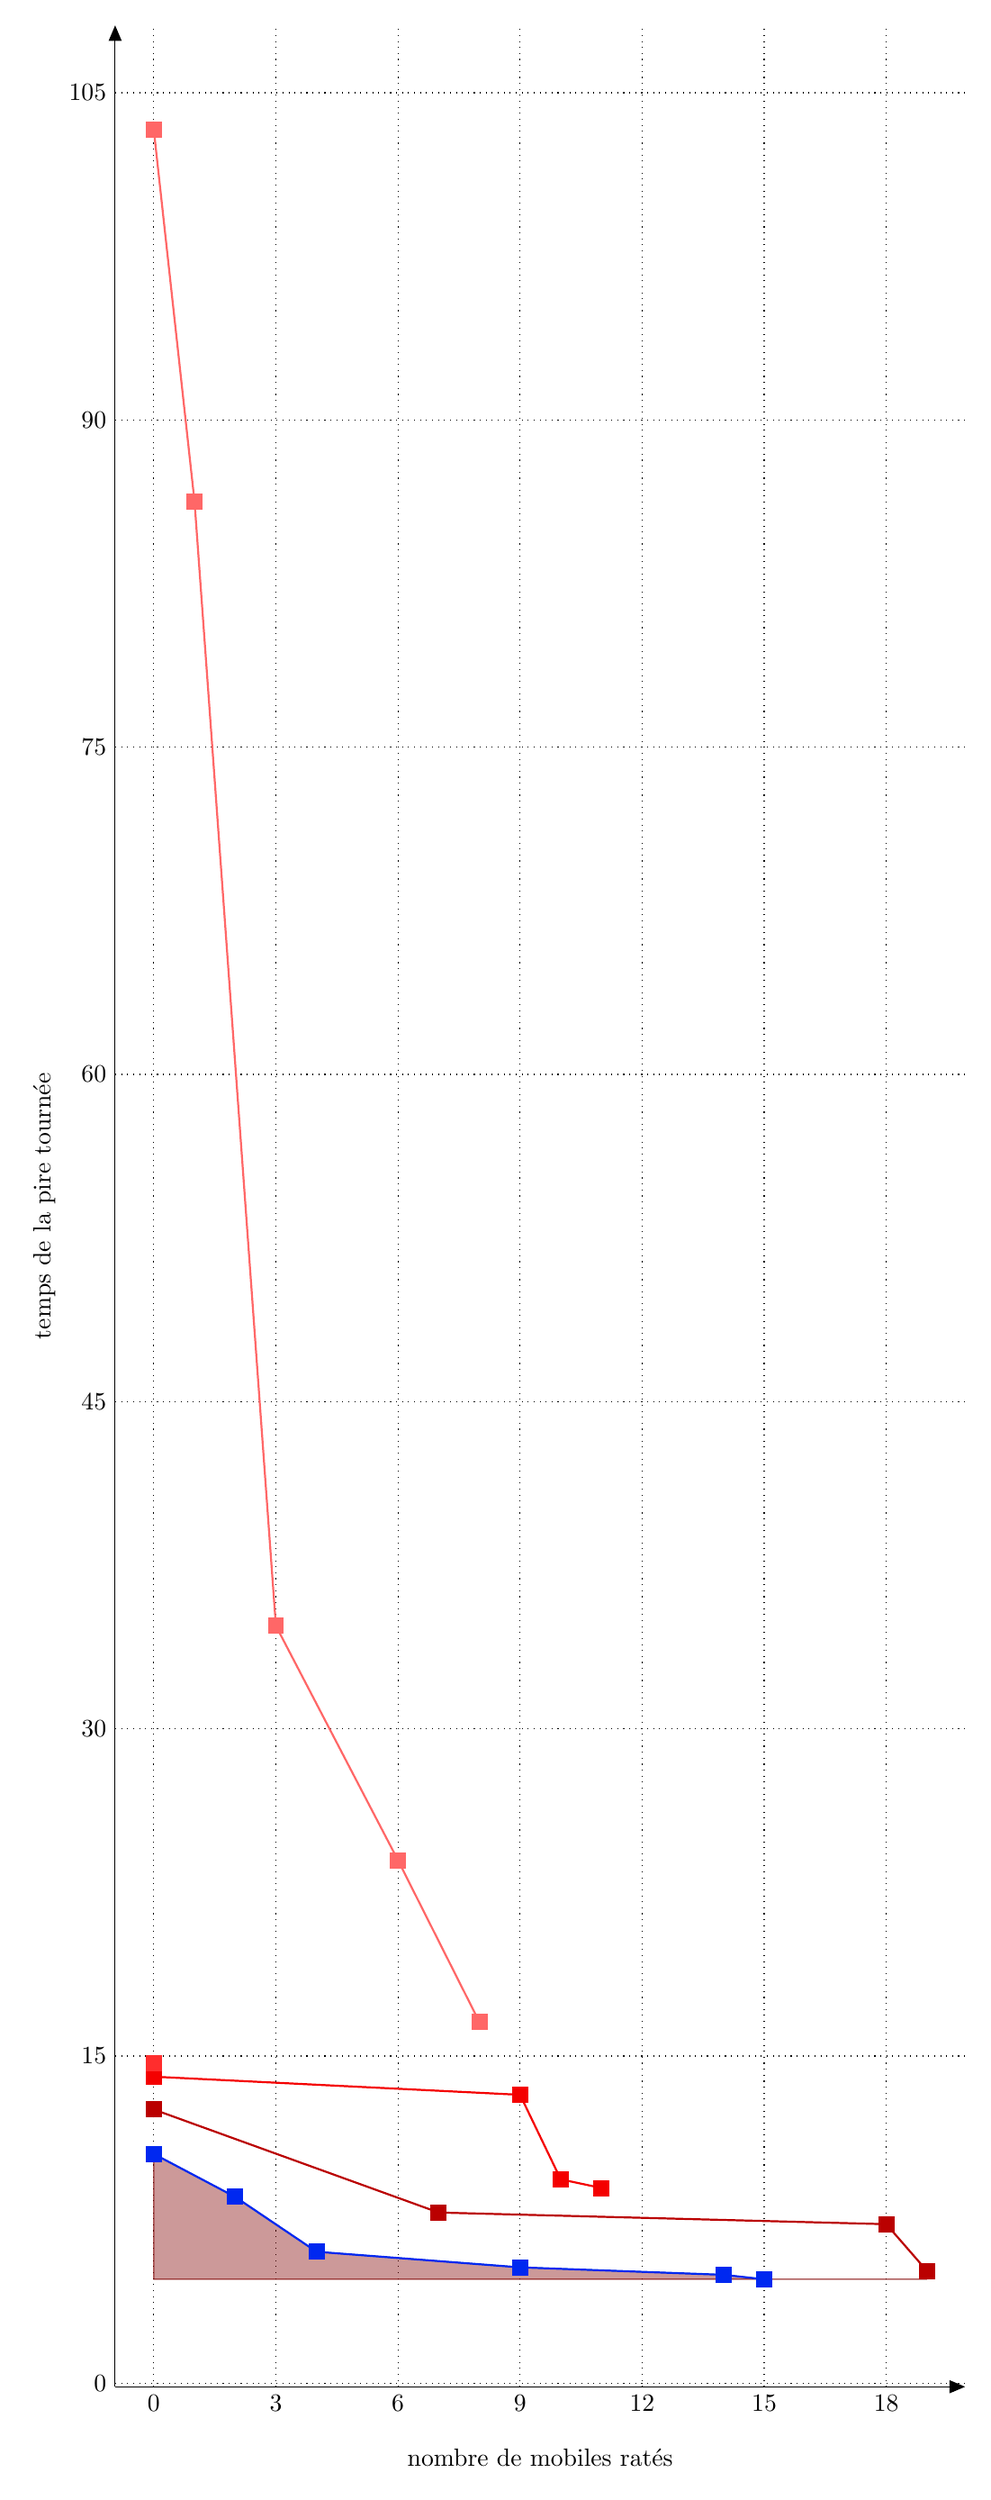
\begin{tikzpicture}[xscale=0.574163,yscale=0.307612]
\draw[xstep=3,ystep=15,thin,dotted,color=Black] (-0.95,-0.161466) grid (19.9365,108.089);
\begin{scope}
  \clip (-0.95,-0.161466) rectangle (19.9365,108.089);
  \definecolor{hvColor}{RGB}{128,0,0}
  \draw[color=hvColor, fill=hvColor, fill opacity=0.4] (0,4.76508) -- (0,10.5108) -- (2,8.5408) -- (4,6.02744) -- (9,5.31211) -- (14,4.96964) -- (15,4.76508) -| (19,4.76508) -- cycle;
  \definecolor{pLineColor}{RGB}{128,0,0}
  \definecolor{pPointColor}{RGB}{0,40,240}
  \draw[thick,color=pPointColor] (0,10.5108) node[draw,color=pPointColor,fill=pPointColor, inner sep = 0pt, minimum size=2mm] {} -- (2,8.5408) node[draw,color=pPointColor,fill=pPointColor, inner sep = 0pt, minimum size=2mm] {} -- (4,6.02744) node[draw,color=pPointColor,fill=pPointColor, inner sep = 0pt, minimum size=2mm] {} -- (9,5.31211) node[draw,color=pPointColor,fill=pPointColor, inner sep = 0pt, minimum size=2mm] {} -- (14,4.96964) node[draw,color=pPointColor,fill=pPointColor, inner sep = 0pt, minimum size=2mm] {} -- (15,4.76508) node[draw,color=pPointColor,fill=pPointColor, inner sep = 0pt, minimum size=2mm] {};
  \definecolor{pLineColor}{RGB}{186,0,0}
  \definecolor{pPointColor}{RGB}{186,0,0}
  \draw[thick,color=pPointColor] (0,12.548) node[draw,color=pPointColor,fill=pPointColor, inner sep = 0pt, minimum size=2mm] {} -- (7,7.82536) node[draw,color=pPointColor,fill=pPointColor, inner sep = 0pt, minimum size=2mm] {} -- (18,7.29127) node[draw,color=pPointColor,fill=pPointColor, inner sep = 0pt, minimum size=2mm] {} -- (19,5.14916) node[draw,color=pPointColor,fill=pPointColor, inner sep = 0pt, minimum size=2mm] {};
  \definecolor{pLineColor}{RGB}{244,0,0}
  \definecolor{pPointColor}{RGB}{244,0,0}
  \draw[thick,color=pPointColor] (0,14.053) node[draw,color=pPointColor,fill=pPointColor, inner sep = 0pt, minimum size=2mm] {} -- (9,13.2225) node[draw,color=pPointColor,fill=pPointColor, inner sep = 0pt, minimum size=2mm] {} -- (10,9.34651) node[draw,color=pPointColor,fill=pPointColor, inner sep = 0pt, minimum size=2mm] {} -- (11,8.95012) node[draw,color=pPointColor,fill=pPointColor, inner sep = 0pt, minimum size=2mm] {};
  \definecolor{pLineColor}{RGB}{255,45,45}
  \definecolor{pPointColor}{RGB}{255,45,45}
  \draw[thick,color=pPointColor] (0,14.6523) node[draw,color=pPointColor,fill=pPointColor, inner sep = 0pt, minimum size=2mm] {};
  \definecolor{pLineColor}{RGB}{255,103,103}
  \definecolor{pPointColor}{RGB}{255,103,103}
  \draw[thick,color=pPointColor] (0,103.296) node[draw,color=pPointColor,fill=pPointColor, inner sep = 0pt, minimum size=2mm] {} -- (1,86.2715) node[draw,color=pPointColor,fill=pPointColor, inner sep = 0pt, minimum size=2mm] {} -- (3,34.722) node[draw,color=pPointColor,fill=pPointColor, inner sep = 0pt, minimum size=2mm] {} -- (6,23.9759) node[draw,color=pPointColor,fill=pPointColor, inner sep = 0pt, minimum size=2mm] {} -- (8,16.5625) node[draw,color=pPointColor,fill=pPointColor, inner sep = 0pt, minimum size=2mm] {};
\end{scope}
\draw[->,>=triangle 45] (-0.95,-0.161466) -- coordinate (x axis mid) (19.9365,-0.161466);
\node[below=1cm,anchor=center] at (x axis mid) {nombre de mobiles ratés};
\foreach \x in {0,3,6,9,12,15,18}
  \draw (\x,-0.161466) -- (\x,-0.161466) node[anchor=north] {\x};
\draw[->,>=triangle 45] (-0.95,-0.161466) -- coordinate (y axis mid) (-0.95,108.089);
\node[left=1cm,rotate=90,anchor=center] at (y axis mid) {temps de la pire tournée};
\foreach \y in {0,15,30,45,60,75,90,105}
  \draw (-0.95,\y) -- (-0.95,\y) node[anchor=east] {\y};
\end{tikzpicture}
\end{document}
